\chapter{Running Heat Transport model with BHEs}

\section{Download and compile the source code}
Currently, the BHE feature is developed in a separate branche of OpenGeoSys, to isolate it from changes of the main OGS development. Once this document is finished and the code is fully verified, it will be merged into the OpenGeoSys main branche and released to the public. For interested readers who would like to have a first look, the code can be downloaded from the following link. 
\par
\url{https://github.com/HaibingShao/ogs5-trunk.git}
\par
Most of the changes are kept under the branch \texttt{borehole\_heat\_exchanger}, and they will be constantly merged into the main branch "develop". 

\subsection{Download the source code}
If you are using the Git command line interface, the code can be obtained by typing in the command line prompt as follows.  
\begin{Verbatim}
C:\haibing_working\ogs>git clone https://github.com/HaibingShao/ogs5-trunk.git
\end{Verbatim}
Or, if you prefer a GUI, I personally recommend to use SourceTree on the Windows platform. After a fresh installation of the software SourceTree, the following interface will appear. 
%%
\begin{figure}
\begin{center}
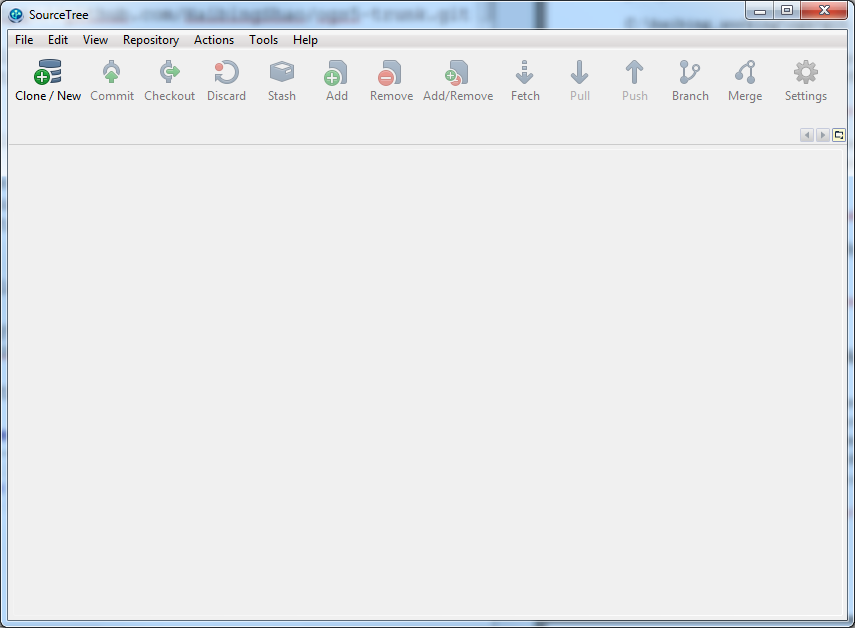
\includegraphics[width=0.8\textwidth]{fig/sourcetree_initial}
\end{center}
\caption{SourceTree window as in the initial stage.}
\label{fig:sourcetree_initial}
\end{figure}
%%
Clicking the button Clone/New in the upper-left corner, you will be asked to give the location of repository. You may use the Github link provided above, or first fork from the above repository and clone from your own repository on Github. 
%%
\begin{figure}
\begin{center}
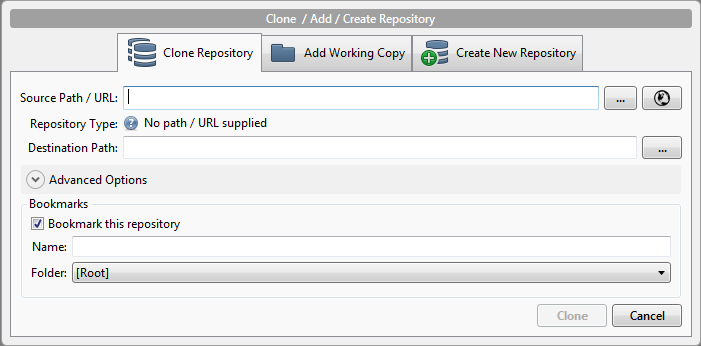
\includegraphics[width=0.6\textwidth]{fig/sourcetree_repo_dialog}
\end{center}
\caption{SourceTree dialog asking for the location of the repository}
\label{fig:sourcetree_repo_dialog}
\end{figure}
%%
After the code has been successfully cloned to your own computer, you will see all history of the development in SourceTree as follows. 
%%
\begin{figure}
\begin{center}
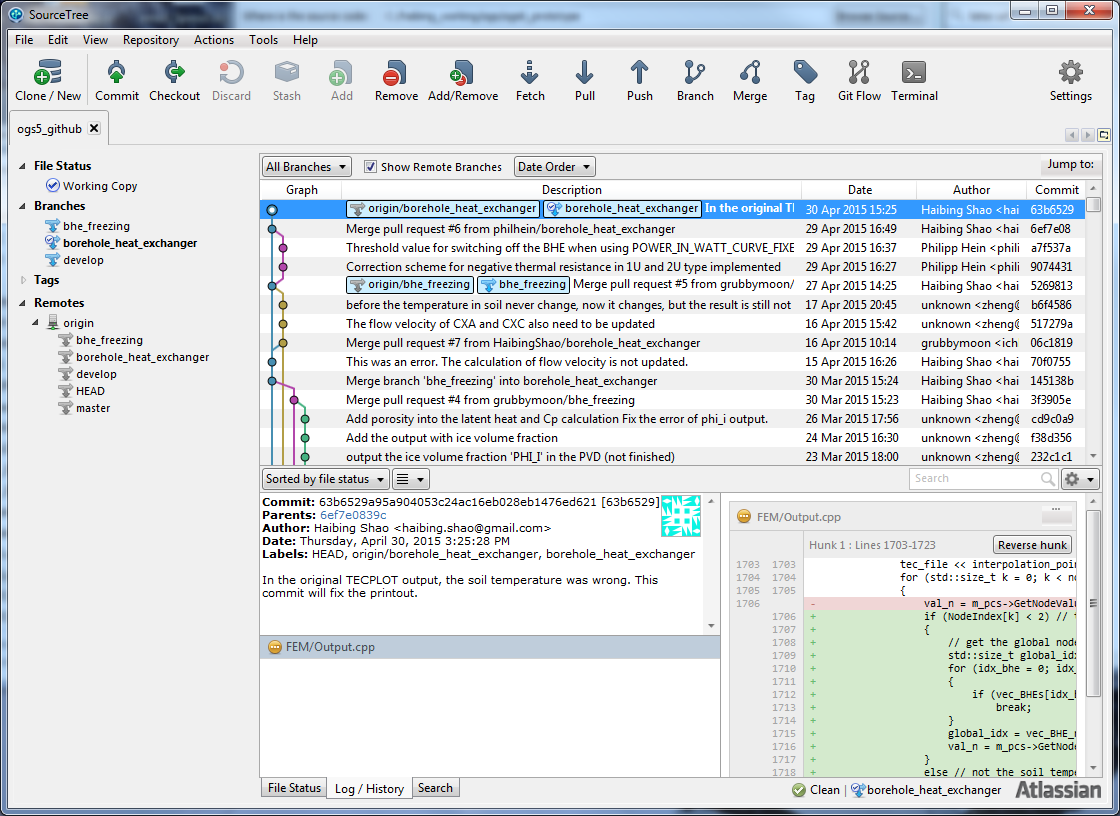
\includegraphics[width=0.8\textwidth]{fig/sourcetree_repo}
\end{center}
\caption{SourceTree window with detailed history of a repository.}
\label{fig:sourcetree_repo}
\end{figure}
%%

\subsection{Using CMake to configure the building project}
Before the compilation of the source code, we need to use the software CMake to generate the configuration and makefiles which are specific to the building environment. Here I am taking CMake version 2.8.12.2 as an example. In the following figure, Cmake GUI was freshly started. First, one needs to define two paths in the CMake GUI. The first one is the folder where the source code of OpenGeoSys is located. The second path refers to the folder where the make files will be generated. 
%%
\begin{figure}
\begin{center}
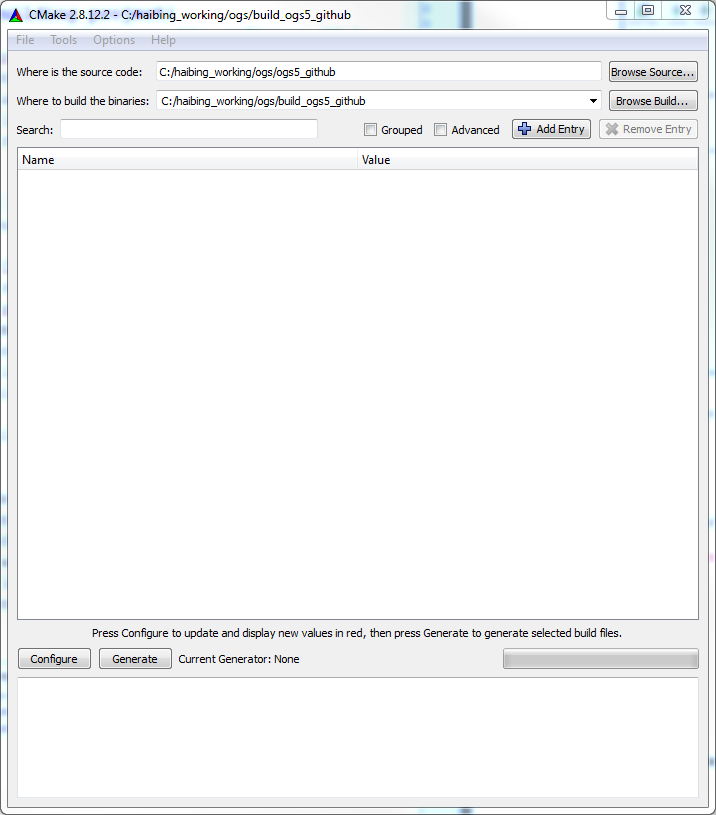
\includegraphics[width=0.6\textwidth]{fig/cmake_initial}
\end{center}
\caption{CMake interface of configuring the build information. }
\label{fig:cmake_initial}
\end{figure}
%%
After clicking on the "Configure" button, CMake will ask several questions, depending on different types of operating system and the compiling tools. In my case, I choose the "Visual Studio 2013 x86" option. Once the configuration has finished, the build options will be demonstrated in the CMake GUI. To build the OpenGeoSys code with BHE features, one only needs to choose the \texttt{OGS\_FEM} option. Finally, once clicking on the "Generate" button, CMake will prepare all makefiles in the build folder. 
%%
\begin{figure}
\begin{center}
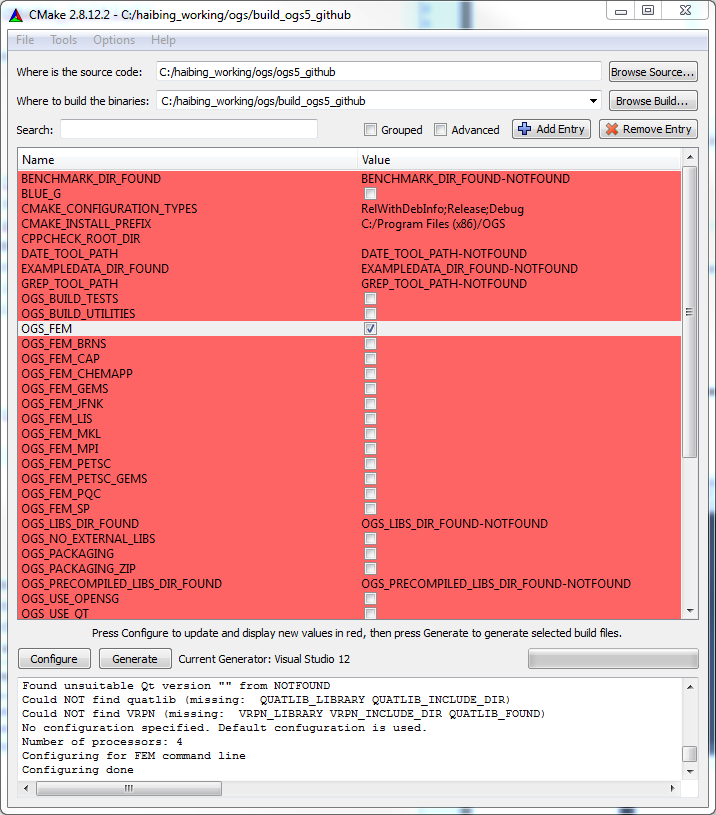
\includegraphics[width=0.6\textwidth]{fig/cmake_configured}
\end{center}
\caption{CMake interface showing different building options. }
\label{fig:cmake_configured}
\end{figure}
%%
\subsection{Compiling the code}
As the author is mainly developing the code with Visual Studio 2013 Express version, the building process will be demonstrated with the same software. Provided the configuration was accomplished by CMake successfully in the previous step, there will be a file named with "OGS.sln" in the build file. Opening this file with Visual Studio will import source code and building configurations into the development environment. 
%%
\begin{figure}
\begin{center}
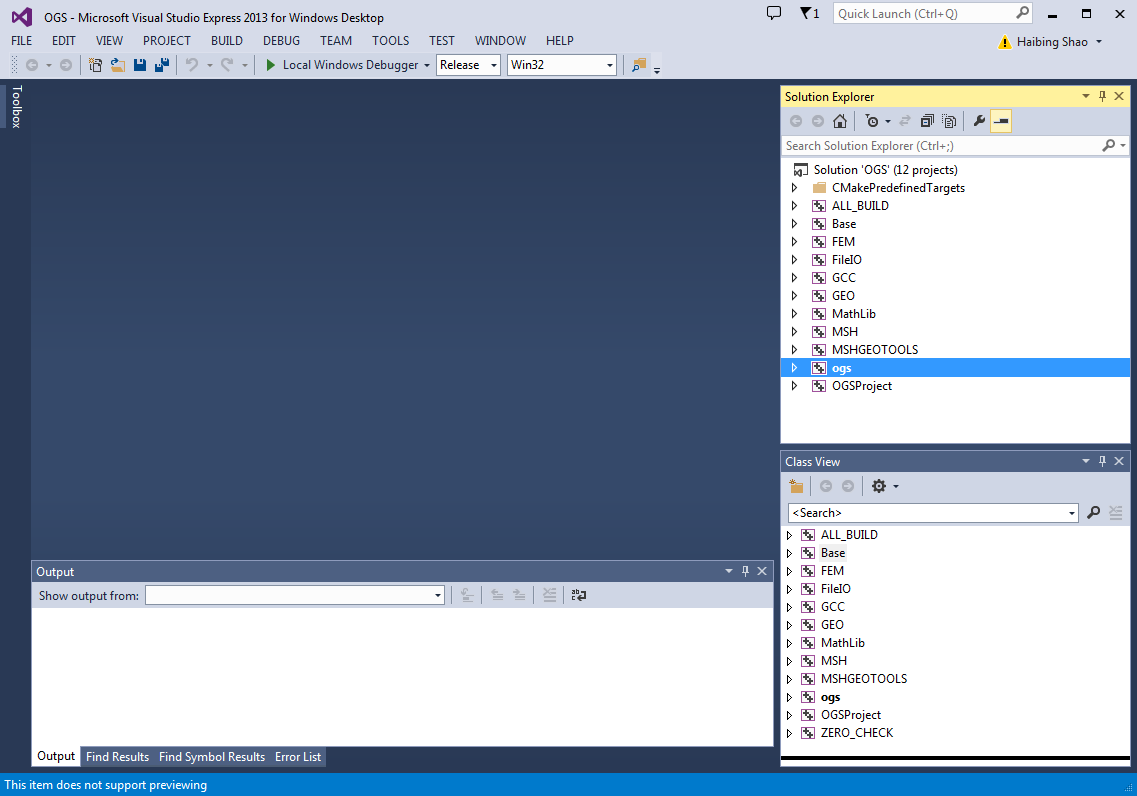
\includegraphics[width=0.8\textwidth]{fig/vs2013exp_ogs}
\end{center}
\caption{Visual Studio interface after opening the OpenGeoSys solution file. }
\label{fig:vs2013exp_ogs}
\end{figure}
%%
To build the source code, choose from the file menu "BUILD", and then click on the first option "Build Solution". It takes a couple of minutes to run the full building process for the first time. After it is finished, the executable files will be found under the bin Debug or bin Release folder, depending on which building mode was chosen. 

\section{Define Heat Transport Process with BHEs}

In the last section, the OpenGeoSys code was successfully compiled and an ogs.exe executable file has been built. In this section, we will introduce the process of setting up a modeling project to simulate heat transport process with borehole heat exchangers.  

\subsection{Process Definition}

Originally, the heat transport simulation in an OpenGeoSys project is performed by defining the process as \texttt{HEAT\_TRANSPORT}. To include the interaction with BHEs, we have introduced a new process named as "\texttt{HEAT\_TRANSPORT\_BHE}". In the following, a PCS file is introduced, with one \texttt{GROUNDWATER\_FLOW} and one \texttt{HEAT\_TRANSPORT\_BHE} process defined in it. 

\begin{Verbatim}[gobble=0, 
                 frame=single, 
                 label=PCS File Definition including Interaction with Borehole Heat Exchangers, 
                 numbers=left]
#PROCESS
 $PCS_TYPE
  GROUNDWATER_FLOW
 $DEACTIVATED_SUBDOMAIN
  1
  1 
#PROCESS
 $PCS_TYPE
  HEAT_TRANSPORT_BHE
 $PRIMARY_VARIABLE
  TEMPERATURE_SOIL
 $BOUNDARY_CONDITION_OUTPUT
#STOP
\end{Verbatim}

\subsection{Deactivated Sub-domains}
In the above PCS file, some readers might have already noticed that there are two numbers given under the key word \texttt{\$DEACTIVATED\_SUBDOMAIN}. The first number "1" on line \#7 means there is one sub-domain deactivated for the \texttt{GROUNDWATER\_FLOW} process, and the second number "1" on line \#8 tells the index of this deactivated domain. So why does the sub-domain "1" need to be turned off? This is because the sub-domain "0" in this project is referring to the soil matrix, while the sub-domain "1" is the borehole heat exchanger. Since the BHE is grouted and impermeable, it is not necessary to calculate groundwater flow through a BHE. Therefore its representative sub-domain is deactivated. 

\subsection{Primary Variables}

From the section \ref{sec:model_concept} and \ref{sec:gov_eqns}, we know that there are multiple primary variables applied in the BHE simulation. In the soil sub-domain primary variable is the soil temperature, while on the BHE they are the temperatures of inlet outlet pipes and their surrounding grout zones. The key words used for these processes, are summerized in Table \ref{tab:pvar_keywords}. In section \ref{sec:temp_output}, when the output is configured, these key words will be used. 

\begin{table}
\caption{Key words used in OGS BHE project for different primary variables. }
\label{tab:pvar_keywords}
\centering
\begin{tabular}{l l }
\hline
Symbols    & Key words  \\
\hline
$T_s$             & \texttt{TEMPERATURE\_SOIL} \\
$T_{i1}$          & \texttt{TEMPERATURE\_IN\_1} \\
$T_{i2}$          & \texttt{TEMPERATURE\_IN\_2} \\
$T_{o1}$          & \texttt{TEMPERATURE\_OUT\_1} \\
$T_{o2}$          & \texttt{TEMPERATURE\_OUT\_1} \\
$T_{g1}$          & \texttt{TEMPERATURE\_G\_1} \\
$T_{g2}$          & \texttt{TEMPERATURE\_G\_2} \\
$T_{g3}$          & \texttt{TEMPERATURE\_G\_3} \\
$T_{g4}$          & \texttt{TEMPERATURE\_G\_4} \\
\hline
\end{tabular}
\end{table}

\section{Geometry of BHEs}

\begin{Verbatim}[gobble=0, 
                 frame=single, 
                 label=Geometry Definition in the GLI File of an OpenGeoSys Project, 
                 numbers=left]
#POINTS
0  0.0 0.0  18.32 $NAME POINT0
1  1.8 0.0  18.32 $NAME POINT1  
2  1.8 1.8  18.32 $NAME POINT2  
3  0.0 1.8  18.32 $NAME POINT3  
4  0.9 0.9  18.32 $NAME POINT4  
5  0.0 0.0  0.0   $NAME POINT5
6  1.8 0.0  0.0   $NAME POINT6  
7  1.8 1.8  0.0   $NAME POINT7  
8  0.0 1.8  0.0   $NAME POINT8  
9  0.9 0.9  0.0   $NAME POINT9  
10 1.14 0.9  18.32 $NAME POINT10  
11 1.14 0.9  0.0   $NAME POINT11  
12 1.34 0.9  18.32 $NAME POINT12  
13 1.34 0.9  0.0   $NAME POINT13
14 1.55 0.9  18.32 $NAME POINT14  
15 1.55 0.9  0.0   $NAME POINT15
16 1.75 0.9  18.32 $NAME POINT16  
17 1.75 0.9  0.0   $NAME POINT17
#POLYLINE
 $NAME
  BHE_1
 $POINTS
   4
   9
#STOP
\end{Verbatim}

As shown in the GLI file above,  "\texttt{BHE\_1}" is refering to a polyline composed of point \#4 and point \#9. To define different BHEs, each BHE in the model has to be given a different polyline in the geometry definition. The geometry names will be used later in the MMP and OUT file as a reference of different BHEs. 

\section{Mesh of BHEs}



\section{Parameters of BHEs}



\section{Output of Temperatures in the BHEs}
\label{sec:temp_output}


\section{Visualization of the Temperatures Evolution}

\subsection{Visualization of Soil Temperatures}

\subsection{Visualization of BHE Temperatures}


